%%%%%
% Presentación Software Libre (UJA)
% Copyright (c) 2016 Nicolás A. Ortega
% Licencia: GNU GPLv3
%%%%%
\documentclass[xetex, mathserif, serif]{beamer}
\usepackage{fontspec}
\usepackage[spanish, es-noquoting]{babel}
\usepackage{graphicx}
\DeclareGraphicsExtensions{.pdf,.png,.jpg,.jpeg}
\usepackage[export]{adjustbox}

\hypersetup{pdfstartview={Fit}} % Fit the presentation to the window by default

% Define theme
\usetheme{Hannover}
\usecolortheme{dove}

% Define title variables
\title{Software Libre}
\subtitle{Libertad en la Era Digital}
\author{Nicolás A. Ortega Froysa}
\institute{Universidad de Jáen}
\date{} % Keep the date blank
\subject{Software Libre}

\begin{document}
% Create the title frame
\frame{\titlepage}

%---------------------------------------------------------------

\begin{frame}
    \frametitle{Contenido}
    \tableofcontents
\end{frame}

%---------------------------------------------------------------

\section{¿Qué es el Software Libre?}
\begin{frame}
    \centering{\Huge ¿Qué es el Software Libre?}
\end{frame}

%---------------------------------------------------------------

\begin{frame}
    \centering
    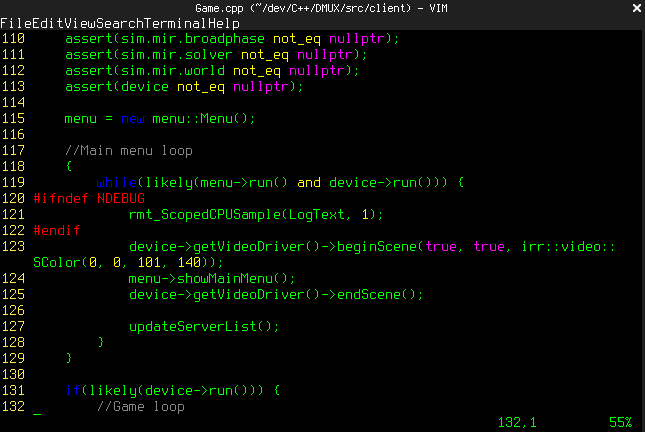
\includegraphics[scale=0.4]{imgs/source}
\end{frame}

%---------------------------------------------------------------

\begin{frame}
    \centering
    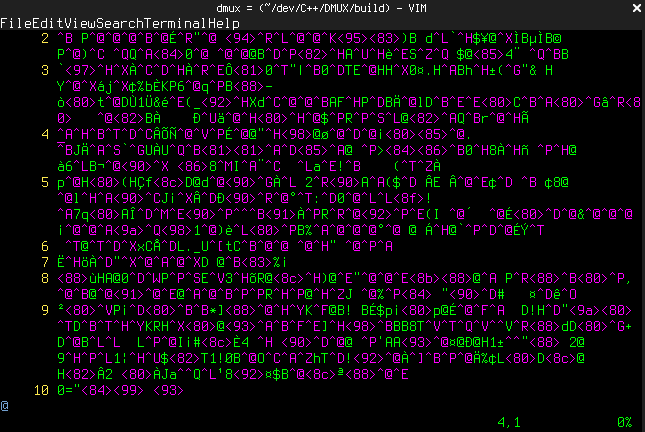
\includegraphics[scale=0.4]{imgs/binary}
\end{frame}

%---------------------------------------------------------------

\subsection{Inicios del Software Libre}
\begin{frame}
    \begin{figure}
        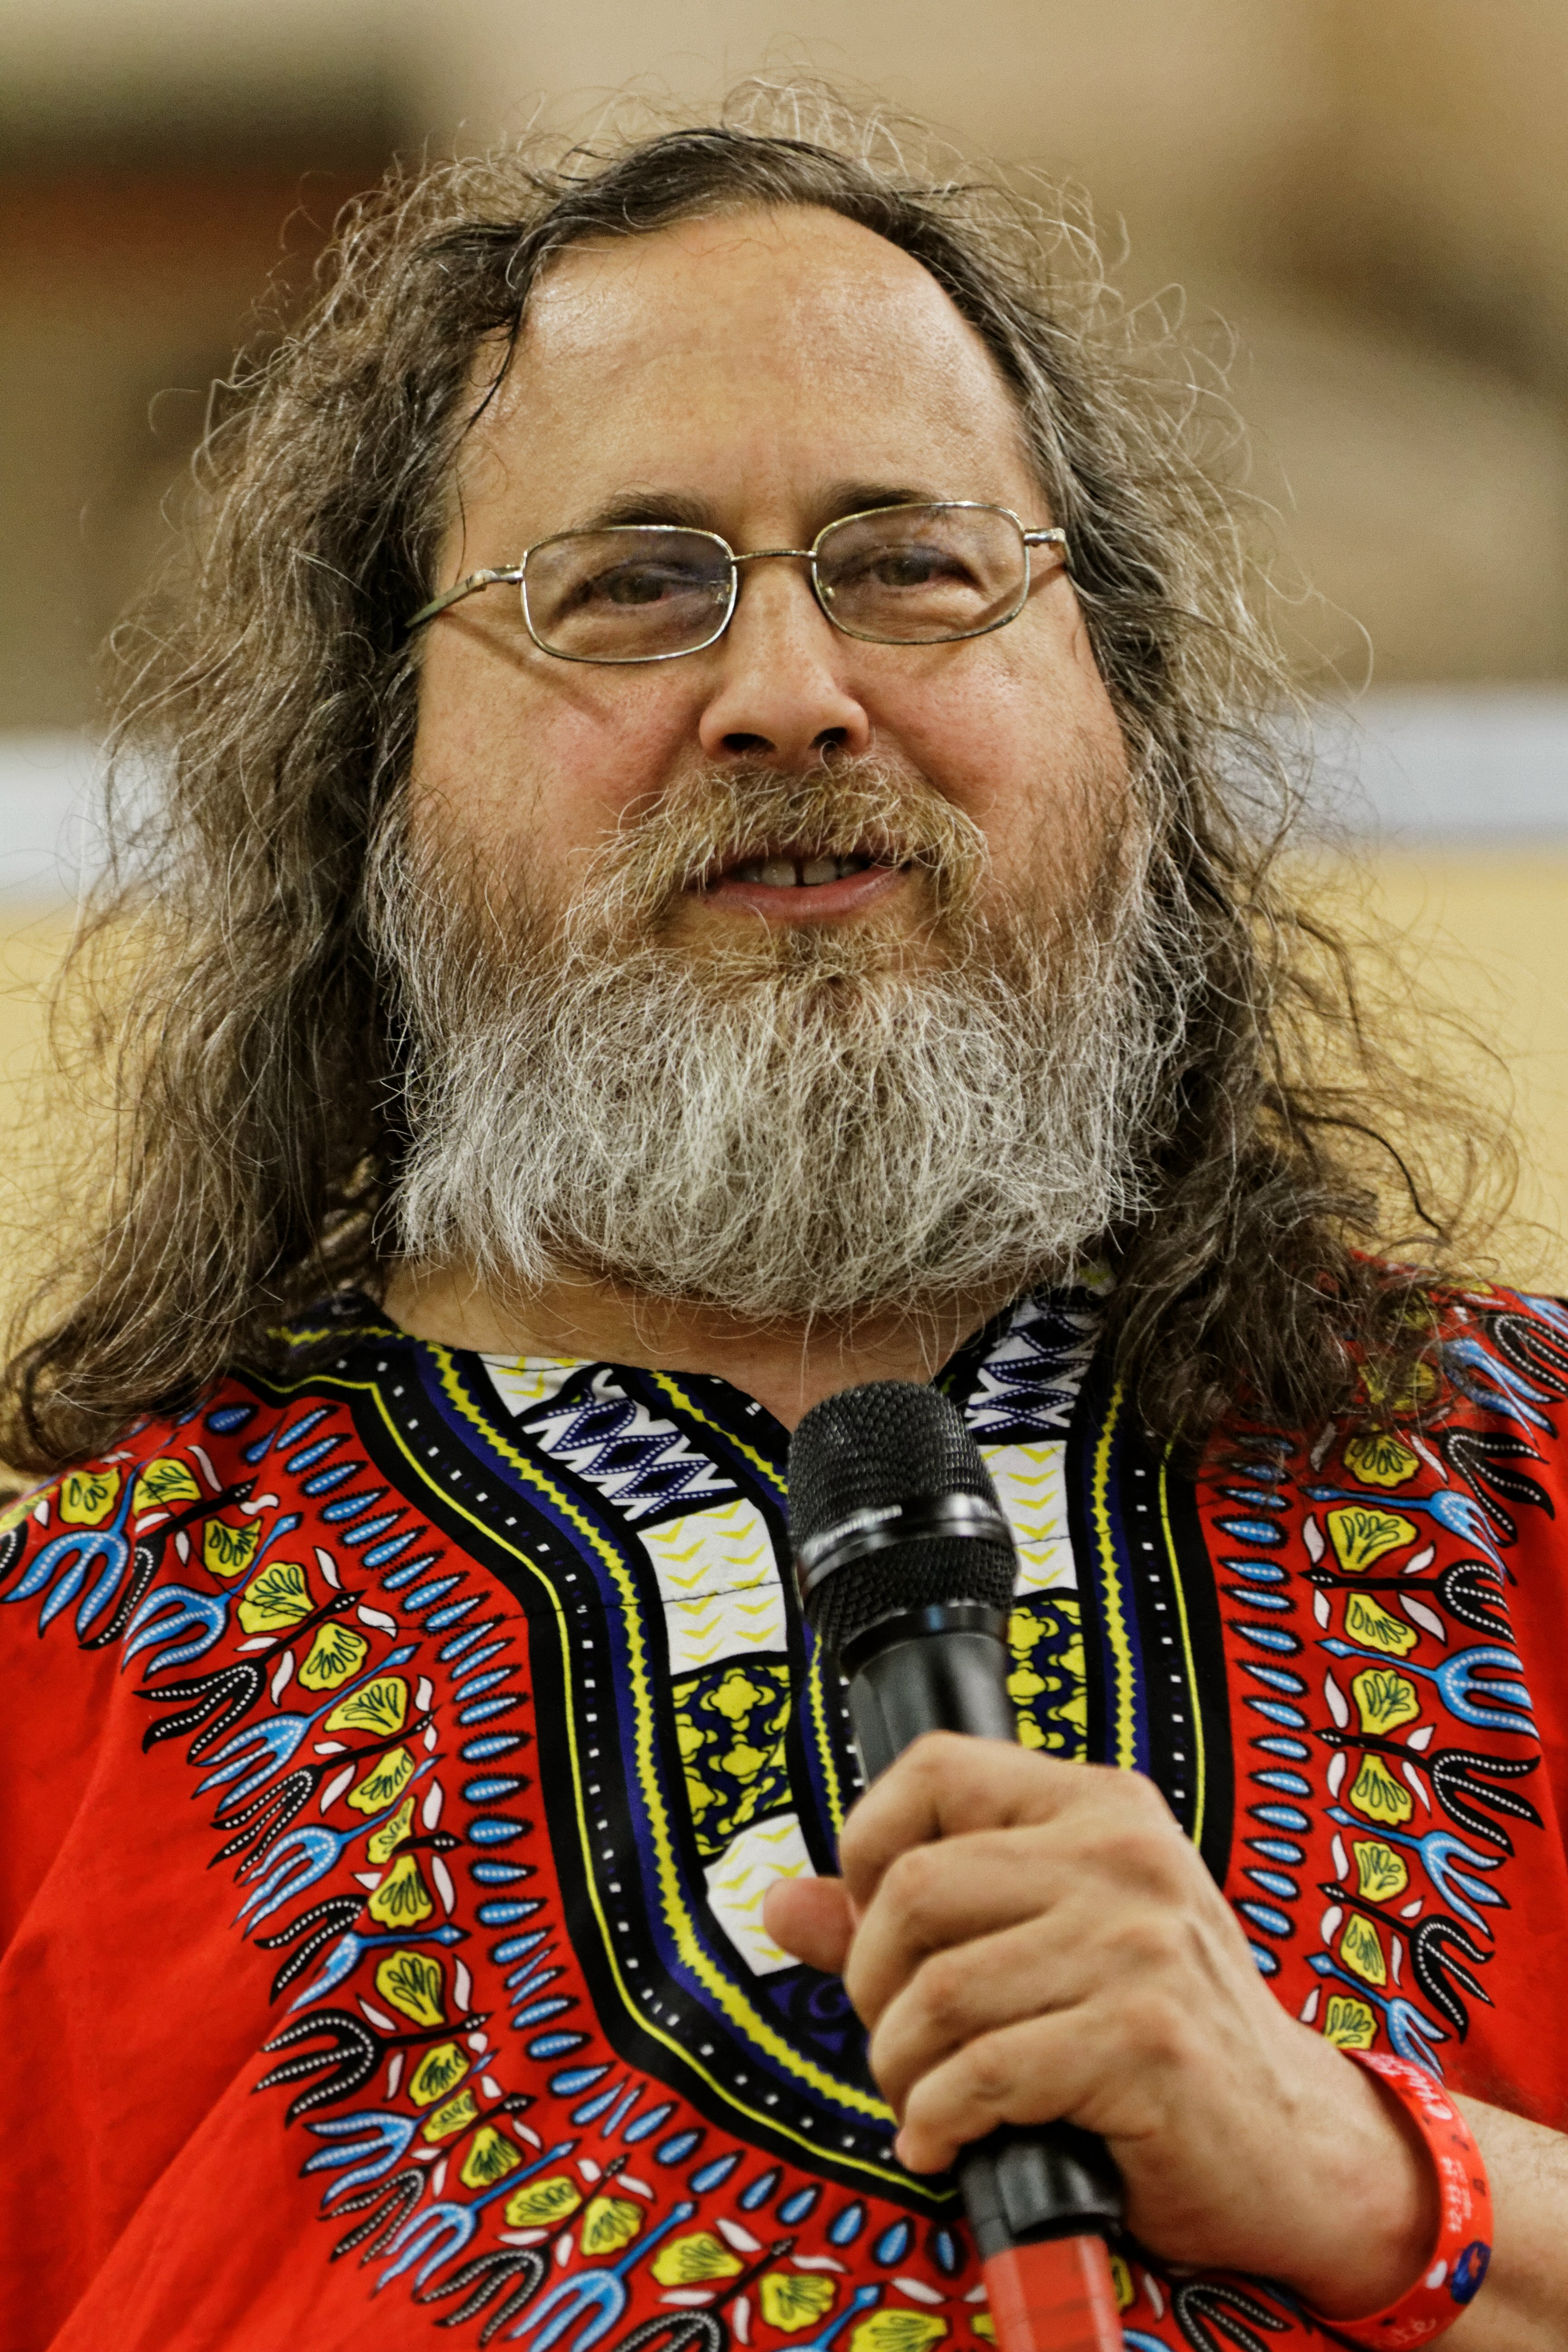
\includegraphics[width=0.4\textwidth]{imgs/rms}
        \pause{}
        \hfill
        
\includegraphics[width=0.4\textwidth]{imgs/gnuu}
    \end{figure}
    \footnotetext[1]{``Conference by Richard Stallman\ldots'', Copyright \copyright{} 2014 Thesupermat, CC-BY-SA 3.0}
    \footnotetext[2]{``gnuu~'', 4chan, N/A}
\end{frame}

%---------------------------------------------------------------

\begin{frame}
    \centering{\Large GNU\linebreak{} (GNU is Not Unix)}
    \begin{figure}
        
\includegraphics[width=0.5\textwidth]{imgs/Heckert_GNU_white}
    \end{figure}
    \footnotetext[1]{``Heckert GNU white'', Copyright \copyright{} Aurelio A. Heckert, CC-BY-SA 3.0}
\end{frame}

%---------------------------------------------------------------

\begin{frame}
    \centering{\Large FSF\linebreak{} (Free Software Foundation)}
    \begin{figure}
        
\includegraphics[width=0.5\textwidth]{imgs/fsf}
    \end{figure}
    \footnotetext[1]{``FSF logo sticker'', Copyright \copyright{} 2010 Free Software Foundation, CC-BY-SA 3.0+}
\end{frame}

%---------------------------------------------------------------

\section{Bibliografía}
\begin{frame}[t]
    \frametitle{Bibliografía}
    \begin{itemize}
        \item ``Free as in Freedom: Richard Stallman's Crusade for Free Software'', Copyright \copyright{} 2002 Sam Williams, GNU Free Document License
    \end{itemize}
\end{frame}

%---------------------------------------------------------------

\section{Licencia}
\begin{frame}
    \frametitle{Licencia}
    Copyright \copyright{} 2016 Nicolás A. Ortega
    \linebreak{}
    \linebreak{}
    Este documento se está licenciada con el GNU GPLv3, y su código fuente se puede encontrar en \url{https://github.com/Deathsbreed/SoftwareLibreUJA}.
    \linebreak{}
    \linebreak{}
    Esta presentación fue posible gracias a \LaTeX, Vim, y la Universidad de Jaén.
\end{frame}

\end{document}
